\documentclass[9pt,pdf,utf8,hyperref={unicode},aspectratio=169]{beamer}

%Привычный шрифт для математических формул
\usefonttheme[onlymath]{serif}
\mode<presentation>
{
    \usetheme{boxes}
    \beamertemplatenavigationsymbolsempty

    \setbeamercovered{transparent}
    \setbeamertemplate{navigation symbols}{}
    
    \setbeamertemplate{footline}[frame number]
    \setbeamertemplate{caption}[numbered]
    % \setbeamersize{text margin left=0.5em, text margin right=0.5em}
}

% Дополнительные библиотеки
\usepackage[T2A]{fontenc}
\usepackage[english, russian]{babel}
\usepackage[utf8]{inputenc}
\usepackage{amsmath,amssymb}
\usepackage{indentfirst}
\usepackage{changepage}
\usepackage{enumerate}
\usepackage{mathtools}
\usepackage{multicol}
\usepackage{multirow}
\usepackage{ragged2e}
\usepackage{multicol}
\usepackage{diagbox}
\usepackage{wrapfig}
\usepackage{comment}
\usepackage{subfig}
\usepackage{array}
\usepackage{color}
\usepackage{tikz}
\usepackage{url}
\usepackage{bm}

\usetikzlibrary{trees}

% Определение дополнительных функций
\DeclareMathOperator*{\plim}{\mathop{plim}}
\DeclareMathOperator{\prob}{\mathbf{P}\!}
\DeclareMathOperator{\arctanh}{arctanh}
\DeclareMathOperator{\mmode}{mode}
\DeclareMathOperator{\rank}{rank}
\DeclareMathOperator{\diag}{diag}
\DeclareMathOperator{\sign}{sign}
\DeclareMathOperator{\cov}{cov}
\DeclareMathOperator{\pow}{pow}
\DeclareMathOperator{\med}{med}

\def\argmin#1{ \mathop{\text{argmin}}\limits_{#1} }
\def\argmax#1{ \mathop{\text{argmax}}\limits_{#1} }

\renewcommand{\leq}{\leqslant}
\renewcommand{\geq}{\geqslant}

\DeclareMathOperator{\FWER}{FWER}
\DeclareMathOperator{\FDR}{FDR}
\newtheorem{Th}{Теорема}
\newtheorem{Def}{Определение}

% Основная часть

\title[Дополнения и обобщения регрессии]{Прикладной статистический анализ данных\\ Дополнения и обобщения регрессии}
\author{Андрей Грабовой}
\date{}

\begin{document}
\tikzstyle{every node}=[draw=black,thick,anchor=west]
\tikzstyle{selected}=[draw=red,fill=red!30]
\tikzstyle{optional}=[dashed,fill=gray!50]

\begin{frame}
    \titlepage
\end{frame}

\section{Дополнения}
\subsection{Пропуски}
\begin{frame}{Неслучайные пропуски}
	Иногда наличие пропуска в $x_j$ информативно:
	
	\begin{itemize}
	\item отказ респондентов отвечать на вопрос
	\item Абрахам Вальд и повреждения самолётов
	\item признак не применим
	\end{itemize}	

	\bigskip

	В таких случаях необходимо:
	\begin{enumerate}
	\item создать новый бинарный признак $$x_{j'}=\begin{cases}1, & x_j=NA, \\ 0, & x_j\neq NA\end{cases}$$
	\item заменить пропущенные значения в $x_j$ на любую не встречающуюся в~$x_j$ константу $c$
	\end{enumerate}
\end{frame}

\begin{frame}{Случайные пропуски}
	Способы борьбы с пропусками в $X$:
	\begin{itemize}
		\item удалить строки, содержащие пропуски (complete cases);
		\item заполнить пропуски (R packages: Amelia, mi, mice):
			\begin{itemize}
			\item по ближайшему объекту
			\item средними или медианами по столбцу
			\item ЕМ-алгоритмом (multiple imputation);
			\end{itemize} 
		\item считать $X^TX$ и $X^Ty$ только по полным парам (available cases):
		$$\left(X^TX\right)_{jl} = \frac1{n}\sum_{i=1}^n x_{ij} x_{il} \approx \frac1{n_{jl}}\sum_{i=1}^n x_{ij} x_{il} \left[x_{ij}\neq NA,  x_{il}\neq NA\right] ,$$
		$n_{jl}$~--- число полных пар.
	\end{itemize}
	
	\bigskip

\end{frame}

\subsection{Интерпретация}
\begin{frame}{Интерпретация регрессионной модели}
	\only<1>{
		\begin{center}
			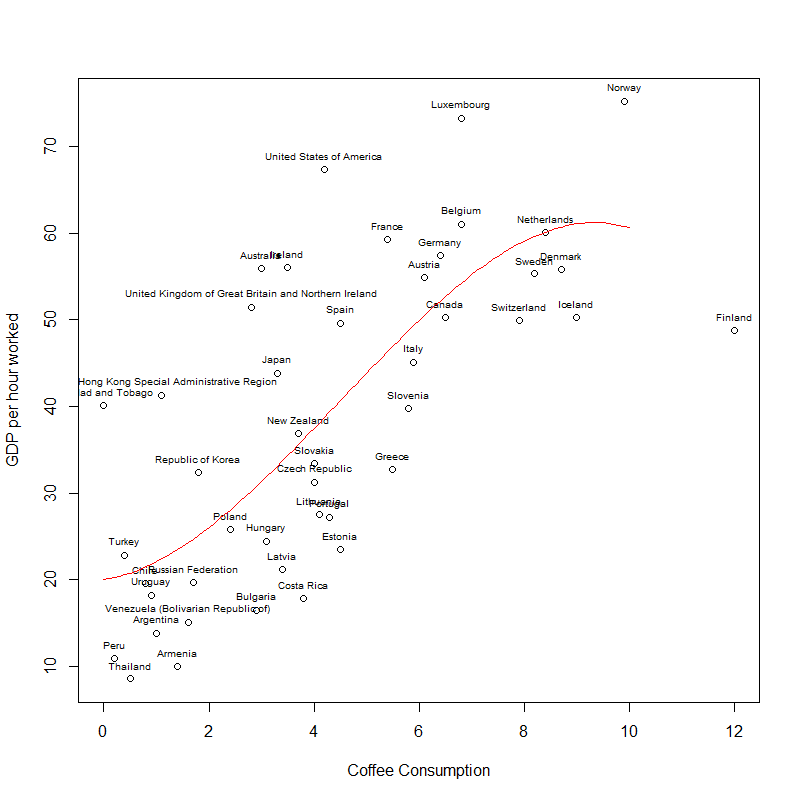
\includegraphics[height=0.9\textheight]{coffee.png}
		\end{center}
	}
	
	\only<2>{
		\begin{center}
			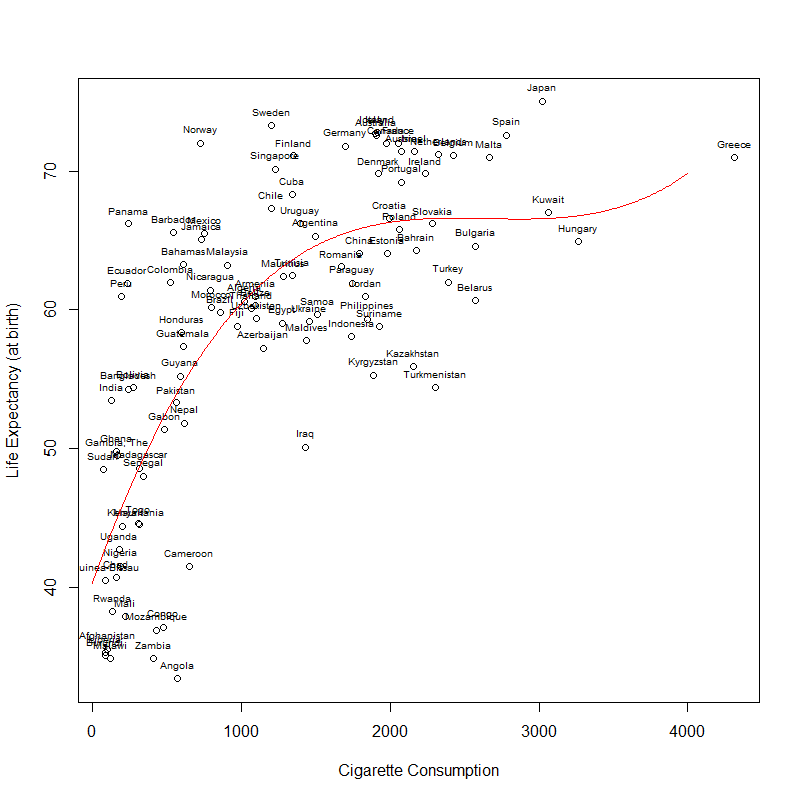
\includegraphics[height=0.9\textheight]{cigarettes.png}
		\end{center}		
	}
	
	\only<3>{
		\begin{center}
			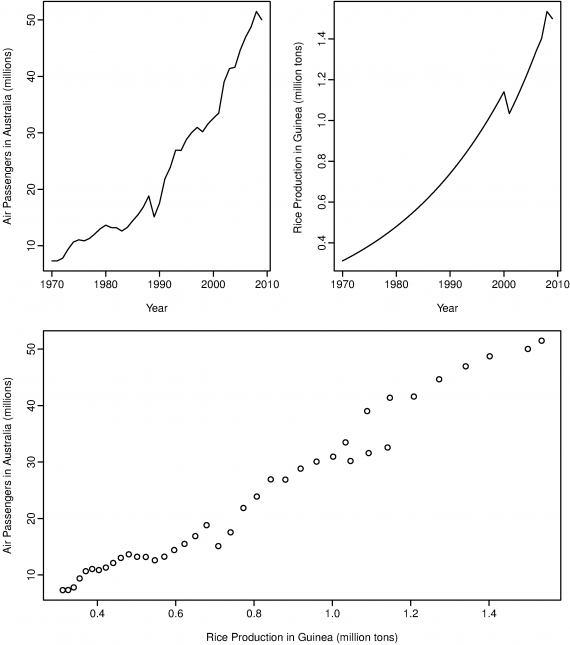
\includegraphics[height=0.9\textheight]{fig_4_spurious-570x645.png}
		\end{center}		
	}
\end{frame}	

\begin{frame}{Интерпретация регрессионной модели}	
		\begin{center}
			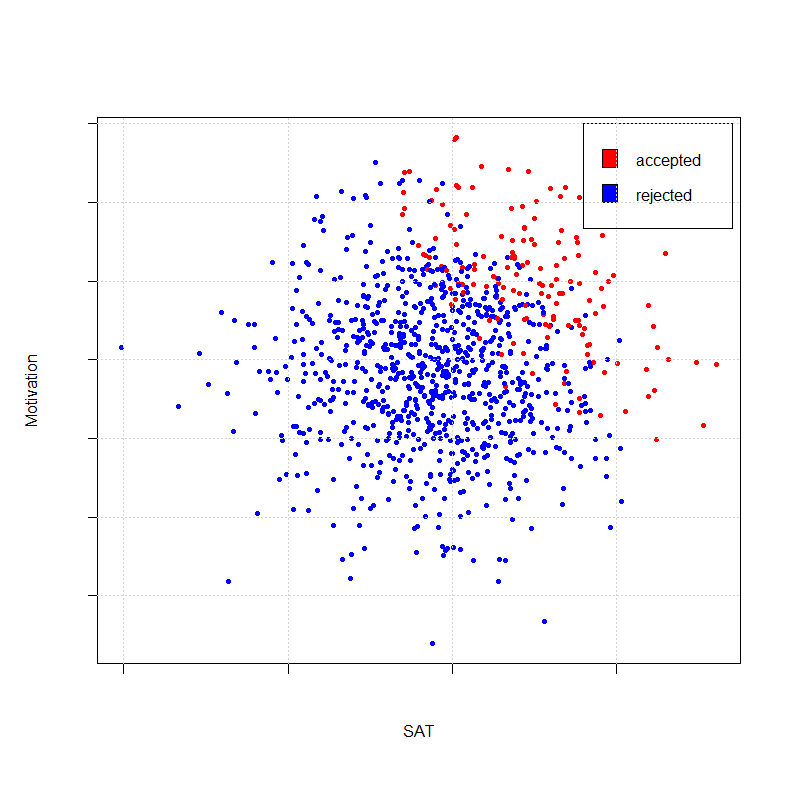
\includegraphics[height=0.95\textheight]{causality.png}
		\end{center}	
\end{frame}	

\begin{frame}[fragile]{Интерпретация регрессионной модели}	
		\begin{center}
			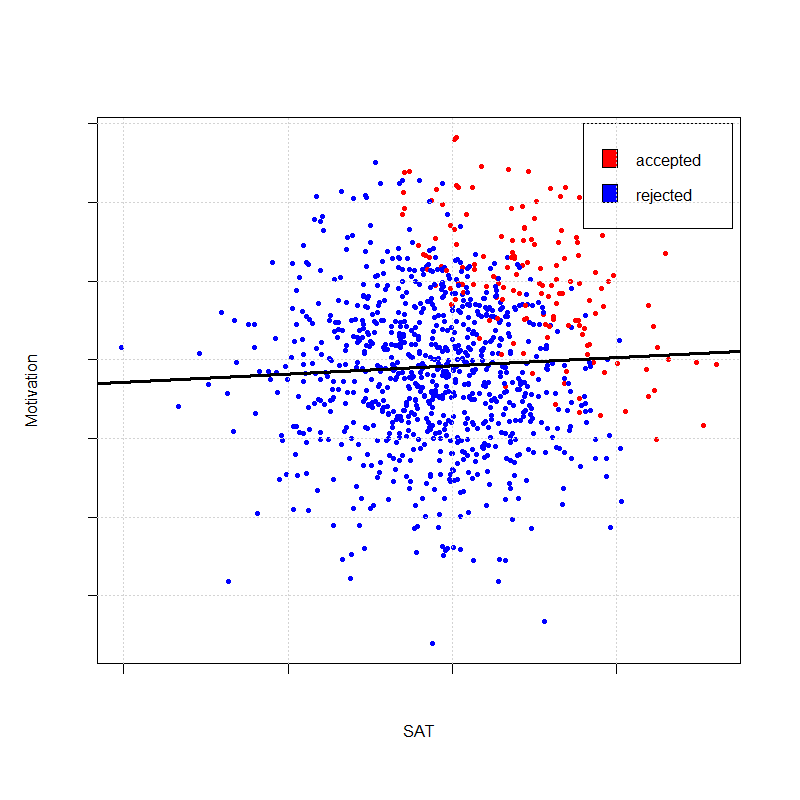
\includegraphics[height=0.5\textheight]{causality1.png}
		\end{center}	
    {\footnotesize
    	\begin{verbatim}
		>summary(lm(motivation~sat, data=school))
		Coefficients:
		            Estimate Std. Error t value Pr(>|t|)  
		(Intercept) -0.07415    0.03211  -2.309   0.0211 *
		sat          0.05204    0.03189   1.632   0.1031  
		---
		Signif. codes:  0 ‘***’ 0.001 ‘**’ 0.01 ‘*’ 0.05 ‘.’ 0.1 ‘ ’ 1
		
		Residual standard error: 1.015 on 998 degrees of freedom
		Multiple R-squared:  0.00266,	Adjusted R-squared:  0.001661 
		F-statistic: 2.662 on 1 and 998 DF,  p-value: 0.1031
    	\end{verbatim}		
	}		
\end{frame}

\begin{frame}[fragile]{Интерпретация регрессионной модели}	
	\begin{center}
		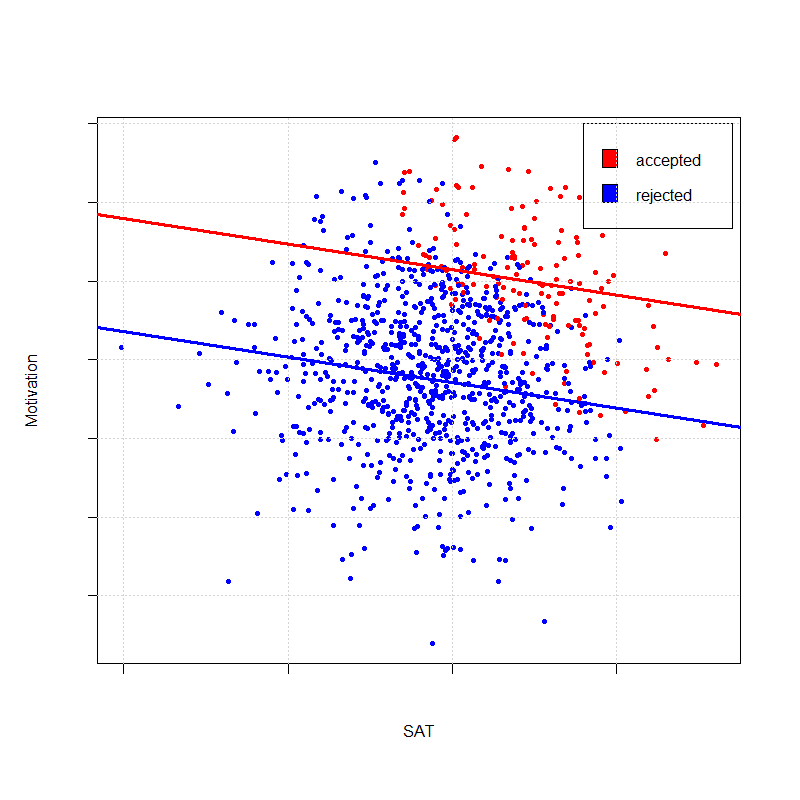
\includegraphics[height=0.5\textheight]{causality2.png}
	\end{center}	
	{\footnotesize
		\begin{verbatim}
		>summary(lm(motivation~sat+acceptance, data=school))
		Coefficients:
		               Estimate Std. Error t value Pr(>|t|)    
		(Intercept)    -0.29246    0.03149  -9.289  < 2e-16 ***
		sat            -0.16248    0.03121  -5.206 2.35e-07 ***
		acceptanceTRUE  1.43688    0.08777  16.372  < 2e-16 ***
		---
		Signif. codes:  0 ‘***’ 0.001 ‘**’ 0.01 ‘*’ 0.05 ‘.’ 0.1 ‘ ’ 1
		
		Residual standard error: 0.9019 on 997 degrees of freedom
		Multiple R-squared:  0.214,	Adjusted R-squared:  0.2124 
		F-statistic: 135.7 on 2 and 997 DF,  p-value: < 2.2e-16
		\end{verbatim}		
	}		
\end{frame}

\begin{frame}[fragile]{Интерпретация регрессионной модели}	
	\begin{center}
		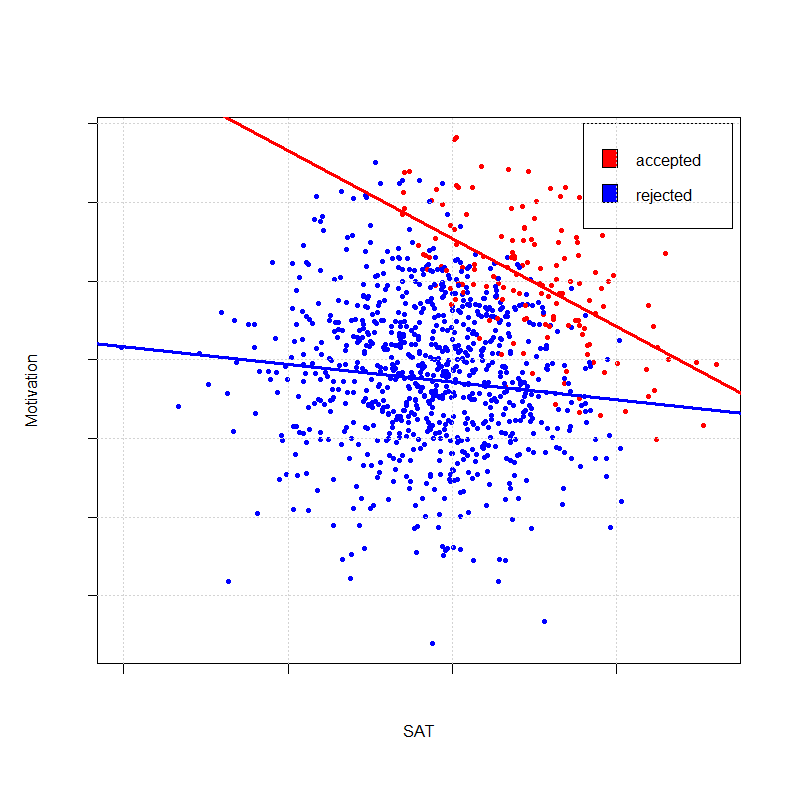
\includegraphics[height=0.5\textheight]{causality3.png}
	\end{center}
		
	\vspace{-5pt}
	
	{\footnotesize
		\begin{verbatim}
		>summary(lm(motivation~sat*acceptance, data=school))
		Coefficients:
		                   Estimate Std. Error t value Pr(>|t|)    
		(Intercept)        -0.28296    0.03124  -9.059  < 2e-16 ***
		sat                -0.11101    0.03284  -3.380 0.000752 ***
		acceptanceTRUE      1.82261    0.12043  15.134  < 2e-16 ***
		sat:acceptanceTRUE -0.44830    0.09692  -4.626 4.23e-06 ***
		---
		Signif. codes:  0 ‘***’ 0.001 ‘**’ 0.01 ‘*’ 0.05 ‘.’ 0.1 ‘ ’ 1
		
		Residual standard error: 0.8928 on 996 degrees of freedom
		Multiple R-squared:  0.2305,	Adjusted R-squared:  0.2282 
		F-statistic: 99.45 on 3 and 996 DF,  p-value: < 2.2e-16
		\end{verbatim}		
	}		
\end{frame}

\subsection{Итог}
\begin{frame}{Требования к решению задачи методом линейной регрессии}
    \begin{itemize}
    \item визуализация данных, анализ распределения признаков (оценка необходимости трансформации), оценка наличия выбросов;
    \item оценка необходимости преобразования отклика и его поиск методом Бокса-Кокса;
    \item визуальный анализ остатков;
    \item проверка гипотез об остатках: нормальность, несмещённость, гомоскедастичность;
    \item отбор признаков с учётом множественной проверки гипотез и~возможной гетероскедастичности;    
    \item анализ необходимости добавления взаимодействий и квадратов признаков;
    \item расчёт расстояний Кука, возможное удаление выбросов, обновление модели;
    \item выводы.
    \end{itemize}
\end{frame}

\section{Обобщённые линейные модели}
\subsection{Постановка}
\begin{frame}{Обобщённая линейная модель}
\only<1>{
    $1,\dots,n$~--- объекты;

    $x_1,\dots,x_k$~--- предикторы;

    $y$~--- отклик;
    
    $$X = \begin{pmatrix}
            x_{10}=1      & x_{11} & \dots  & x_{1k} \\
            \vdots & \vdots & \ddots & \vdots \\
            x_{n0}=1      & x_{n1} & \dots  & x_{nk}
          \end{pmatrix};
    \qquad
    y =  \begin{pmatrix}
            y_1 \\ \vdots \\ y_n
         \end{pmatrix};
    $$
    
    \bigskip
    
    регрессионная модель:
    $$\mathbb{E}\left(y\left|X\right.\right) \equiv \mu = f\left(x_1,\dots,x_k\right);$$
    
    линейная регрессионная модель:
    $$\mu  = X\beta;$$
    
    обобщённая линейная регрессионная модель (GLM): 
    $$g\left(\mu\right) = X\beta, \;\;\; \mu = g^{-1}\left(X\beta\right),$$
    
    $g\left(x\right)$~--- связующая функция~--- позволяет ограничить диапазон предсказываемых для $\mu$ значений.
    }
    
    \only<2>{
    В обычной линейной модели используется предположение о~нормальности отклика: $$y\left|X\right.\sim N\left(X\beta,\sigma^2\right).$$
    
    В обобщённой линейной модели распределение $y$ берётся из~экспоненциального семейства:
    $$f(y, \theta, \phi) = \exp \left( \frac{y\theta - b\left(\theta\right)}{a\left(\phi\right)} + c\left(y,\phi\right)\right).$$
    
    \begin{center}
    \begin{tabular}{|c|c|c|c|}
        \hline
                               & $Pois\left(\lambda\right)$ & $Bin\left(N,p\right)$          & $N\left(\mu,\sigma^2\right)$ \\\hline
        $a\left(\phi\right)$   & $1$                        & $1$                            & $\sigma^2$ \\
        $b\left(\theta\right)$ & $e^\theta$                 & $n\ln\left(1+e^\theta\right)$ & $\theta^2/2$ \\
        $c\left(y,\phi\right)$ & $\ln y!$                  & $\ln C_n^y$                   & $\frac1{2} \left(\frac{y^2}{\phi} + \ln \left(2\pi\phi\right)\right)$\\
		$g\left(x\right)$      & $\ln x$                   & $\ln\frac{x}{1-x}$            & $x$ \\
		$g^{-1}\left(x\right)$ & $e^x \in \left[0,\infty\right)$ & $\frac{e^x}{1+e^x} \in \left[0,1\right]$ & $x \in \mathbb{R}$ \\\hline
    \end{tabular}
    \end{center}    
    }
\end{frame}

\subsection{Свойства}
\begin{frame}{Оценка параметров GLM}
	$\hat{\beta}$:
        \begin{itemize}
	        \item оценивается методом максимального правдоподобия;
        	\item существует и единственна,
        	\item находится численно 
        	\begin{itemize}
        		\item методом Ньютона"=Рафсона (Newton-Raphson method)
        		\item методом оценок Фишера (Fisher scoring method)
        	\end{itemize}
        	\item состоятельна, асимптотически эффективна, асимптотически нормальна.
        \end{itemize}
    Итерационный процесс вычисления $\hat{\beta}$ может не сойтись, если $k$ слишком велико относительно~$n$.
     
    \bigskip
        
    $$\mathbb{D}\hat{\beta} = I^{-1}\left(\hat{\beta}\right),$$
    $I\left(\beta\right) \in \mathbb{R}^{\left(k+1\right)\times\left(k+1\right)}$~--- информационная матрица Фишера~--- матрица вторых производных логарифма правдоподобия  $L\left(\beta\right)$.       
\end{frame}

\begin{frame}{Доверительные интервалы}
    Для отдельного коэффициента $\beta_j$:
    $$\hat{\beta}_j \pm z_{1-\alpha/2} \sqrt{\left(I^{-1} \left(\hat{\beta}\right)\right)_{jj}}.$$

    \bigskip

    Для $g\left(\mathbb{E}\left(y\left|x_0\right.\right)\right)$~--- преобразованного матожидания отклика на новом объекте $x_0$:
    $$x_0^T \hat{\beta} \pm z_{1-\alpha/2} \sqrt{x_0^T I^{-1}\left(\hat{\beta}\right) x_0}.$$

    \bigskip

    Для матожидания отклика на новом объекте $x_0$:
    $$\left[g^{-1}\left(x_0^T \hat{\beta} - z_{1-\alpha/2} \sqrt{x_0^T I^{-1}\left(\hat{\beta}\right) x_0}\right), 
            g^{-1}\left(x_0^T \hat{\beta} + z_{1-\alpha/2} \sqrt{x_0^T I^{-1}\left(\hat{\beta}\right) x_0}\right)\right].$$
\end{frame}

\begin{frame}
    \frametitle{Критерий Вальда}
    \begin{center}
        \begin{tabular}{rl}
            нулевая гипотеза:               & $H_0\colon \beta_j=0$ \\
            альтернатива:                   & $H_1\colon \beta_j<\neq>0$ \\
            статистика:                     & $T = \frac{\hat{\beta}_j}{ \sqrt{\left(I^{-1}\left(\hat{\beta}\right)\right)_{jj}} }$ \\
            нулевое распределение:          & $N(0,1)$\\
        \end{tabular}
        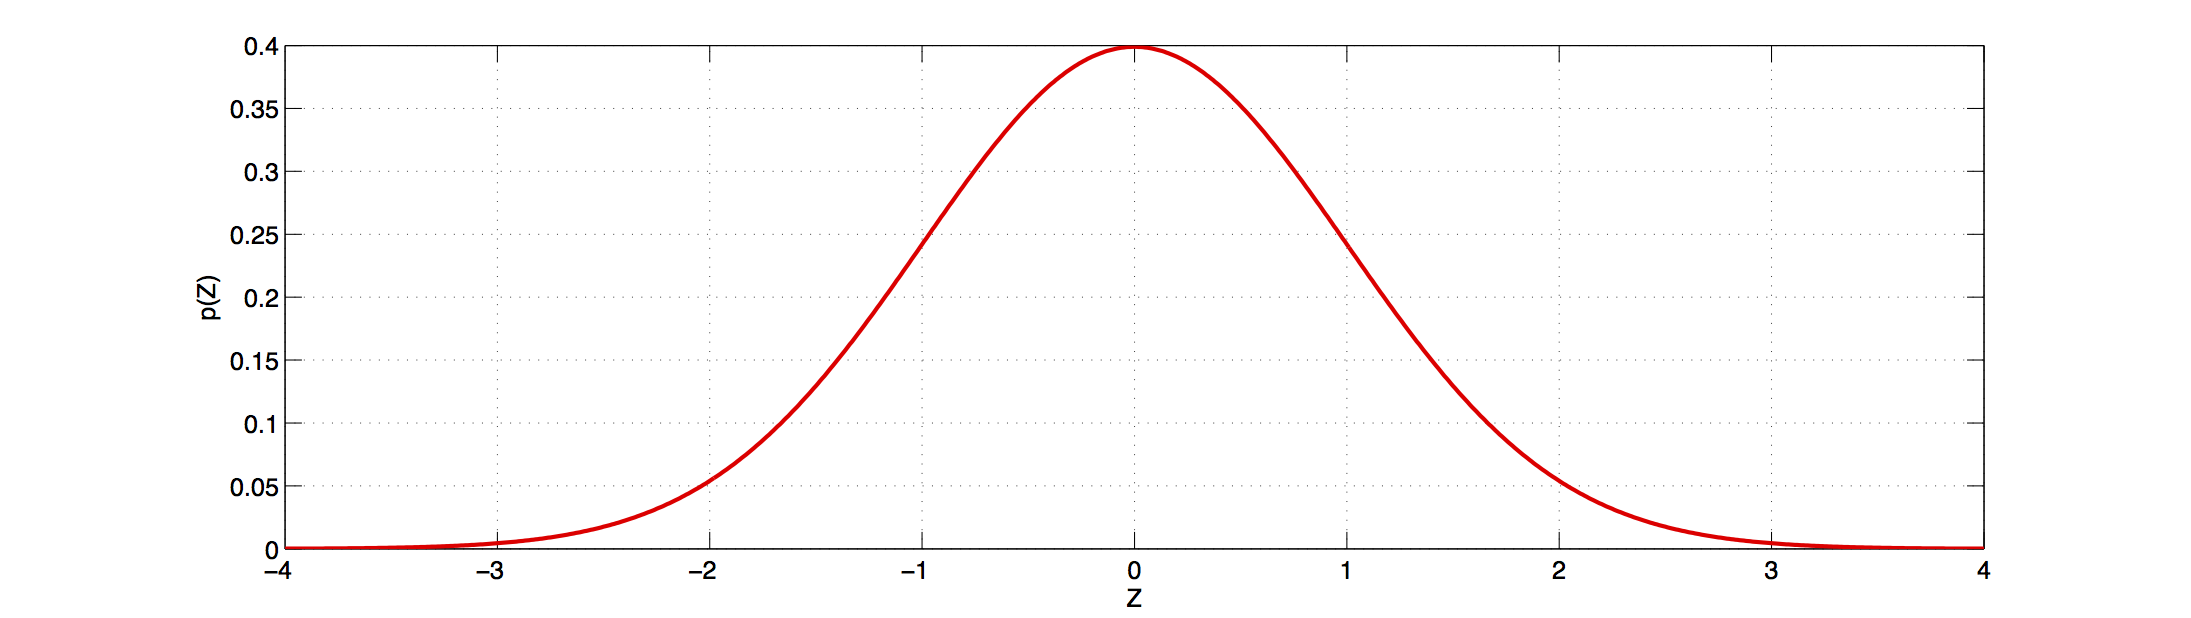
\includegraphics[width=0.85\textwidth]{norm.png}
    \end{center}
\end{frame}

\begin{frame}{Критерий отношения правдоподобия}
    $$\underset{n\times (k+1)}{X} = \left(\underset{n\times \left(k+1-k_1\right)}{X_1} , \underset{n\times k_1}{X_2}\right); \quad \underset{(k+1)\times 1}{\beta^T} = \left(\underset{\left(k+1-k_1\right)\times 1}{\beta_1^T}, \underset{k_1\times 1}{\beta_2^T} \right)^T;$$
    \begin{center}
        \begin{tabular}{rl}
            нулевая гипотеза:               & $H_0\colon \beta_2=0$ \\
            альтернатива:                   & $H_1\colon H_0$ неверна\\
            статистика:                     & $G = 2 \left(L_{r} - L_{ur}\right)$\\
            нулевое распределение:          & $\chi^2_{k_1}$\\
        \end{tabular}
        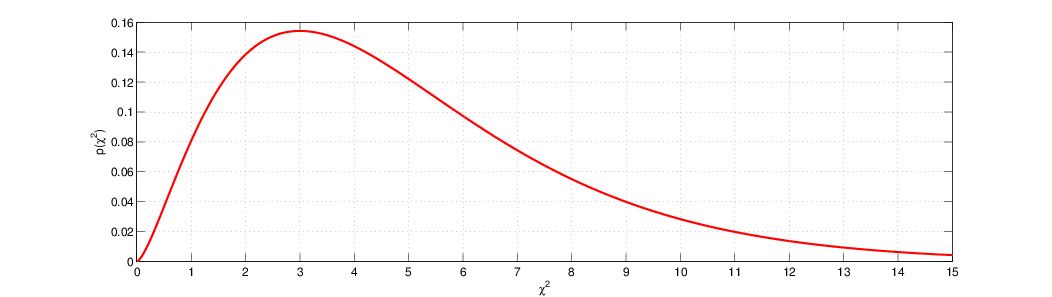
\includegraphics[width=0.85\textwidth]{chi2.png}   
    \end{center}
\end{frame}

\begin{frame}{Связь между критериями Вальда и отношения правдоподобия}
    При $k_1=1$ критерии Вальда и отношения правдоподобия не~эквивалентны, в отличие от случая линейной регрессии, когда в этом случае достигаемые уровни значимости критериев Стьюдента и Фишера совпадают.

    \bigskip

   При больших $n$ разница между критериями невелика, но~в~случае, когда их показания расходятся, рекомендуется смотреть на~результат критерия отношения правдоподобия.
\end{frame}


\begin{frame}{Меры качества моделей}
\only<1>{
    \textbf{Остаточная аномальность} (residual deviance):
    $$D_{res} = 2(L_{sat} - L_{fit})$$
    Где $L_{sat}$ -- насыщенная (saturated) модель, имеющая число параметров равное числу объектов.
    
    Аномальность~--- аналог RSS в линейной регрессии; при добавлении признаков она не может убывать.

    \medskip

    Для сравнения моделей с разным числом признаков можно использовать \textbf{информационные критерии}:
    
    \begin{enumerate}
    \item 	$AIC$~--- информационный критерий Акаике:
    	$$AIC = -2L + 2\left(k+1\right);$$
  
	\item $AICc$~--- он же с поправкой на случай небольшого размера выборки;
	$$AICc = -2L + \frac{2k\left(k+1\right)}{n-k-1};$$	
	
	\item  $BIC$ ($SIC$)~--- байесовский (Шварца) информационный критерий:
	$$BIC = -2L + \ln n\left(k+1\right).$$	
	 \end{enumerate}
}
\only<2>{
	\begin{itemize}
		\item $AIC<AICc$
		\item $BIC>AIC$ при $n\geq 8$
		\item выбор модели по $BIC$ приводит к состоятельным оценкам~--- с ростом $n$ вероятность выбора верного подмножества признаков стремится к 1
		\item минимизация $AIC$ асимптотически даёт модель с наименьшей среднеквадратичной ошибкой предсказания
		\item модели со значением информационного критерия на расстоянии двух единиц от значения лучшей модели можно считать неотличимыми от лучшей
	\end{itemize}
	
}
\end{frame}

\section{Бинарный отклик}
\subsection{Постановка}
\begin{frame}{Бинарный отклик: постановка задачи}
    \textbf{Задача}: оценить влияние одного или нескольких признаков на~наступление какого-либо события и оценить его вероятность.

    \bigskip

    $1,\dots,n$~--- объекты;

    $x_1,\dots,x_k$~--- предикторы;

    $y$~--- отклик, $y_i \in \left\{0,1\right\}$.

	\bigskip  
	
	Хотим найти такой вектор $\beta$, что $$\mu = \mathbb{E} \left(y\left|X\right.\right) = P\left(y=1\left|X\right.\right) \equiv \pi(x) \approx X\beta.$$
\end{frame}

\begin{frame}{Примеры}
    Неповторяемый эксперимент со случайными уровнями фактора:
    
    построение кривой спроса, $x_i$~--- цена  товара, $y_i$~--- согласие купить товар. 
    \begin{center}
        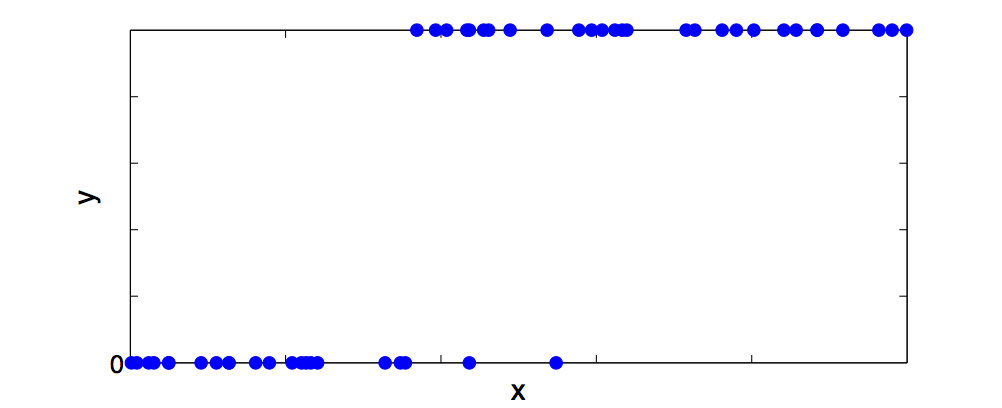
\includegraphics[width=0.3\textwidth]{ex2.png}
    \end{center}

	\bigskip

    Повторяемый эксперимент с фиксированными уровнями фактора:
    
    разработка пестицидов, $x_i$~--- доза пестицида, $y_i$~--- смерть вредителя.    
    
    \begin{center}
        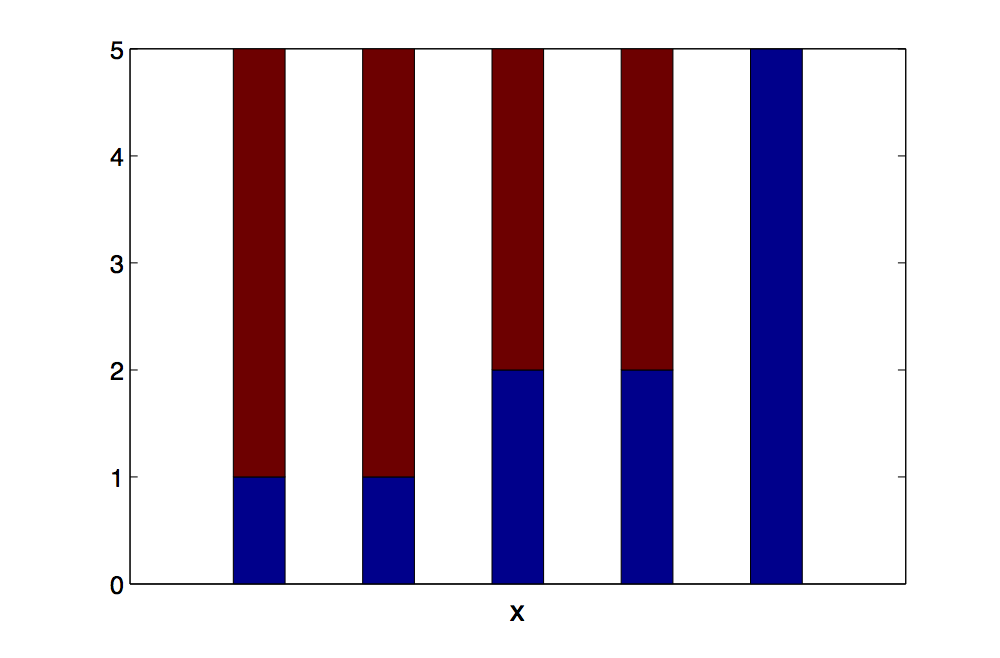
\includegraphics[width=0.3\textwidth]{ex1.png}
    \end{center}
    
    \vspace{-10pt}
    
    $\Longrightarrow$ логистическая регрессия может также использоваться для~моделирования $y \in \left[0,1\right].$    
\end{frame}

\subsection{Логит}
\begin{frame}{Параметризация}
%    \only<1>{
%    Линейная регрессия: $$\pi\left(x\right) = \beta_0 + \beta_1 x + \varepsilon.$$
%    \begin{itemize}
%    \item Оценка вероятности может выходить за $[0,1].$
%    \item В линейной регрессии $y = \mathbb{E}\left(y\left|x\right.\right) + \varepsilon$, и МНК-оценка $\beta$ хороша, когда $\varepsilon \sim N\left(0,\sigma\right)$. Здесь же, если $y = \pi\left(x\right) + \varepsilon$, то $\varepsilon = 1 - \pi(x)$ или $\varepsilon = \pi(x)$, и МНК-оценка будет плохой.
%    \end{itemize}
%
%    \bigskip
%
%    Нужно такое нелинейное преобразование $$g\left(\pi\left(x\right)\right) = \beta_0 + \beta_1x + \varepsilon,$$ чтобы:
%    }
    Логит:
\[
     g\left(\pi\left(x\right)\right) = \ln \frac{\pi\left(x\right)}{1-\pi\left(x\right)} = \beta_0 + \beta_1x + \varepsilon,
\]
\[
    \hat{\pi}\left(x\right) = \frac{e^{\hat{g}\left(x\right)}}{1+e^{\hat{g}\left(x\right)}} = \frac{e^{\hat{\beta}_0 + \hat{\beta}_1x }}{1 + e^{\hat{\beta}_0 + \hat{\beta}_1x }}.
\]

    \only<1>{
    \begin{center}
        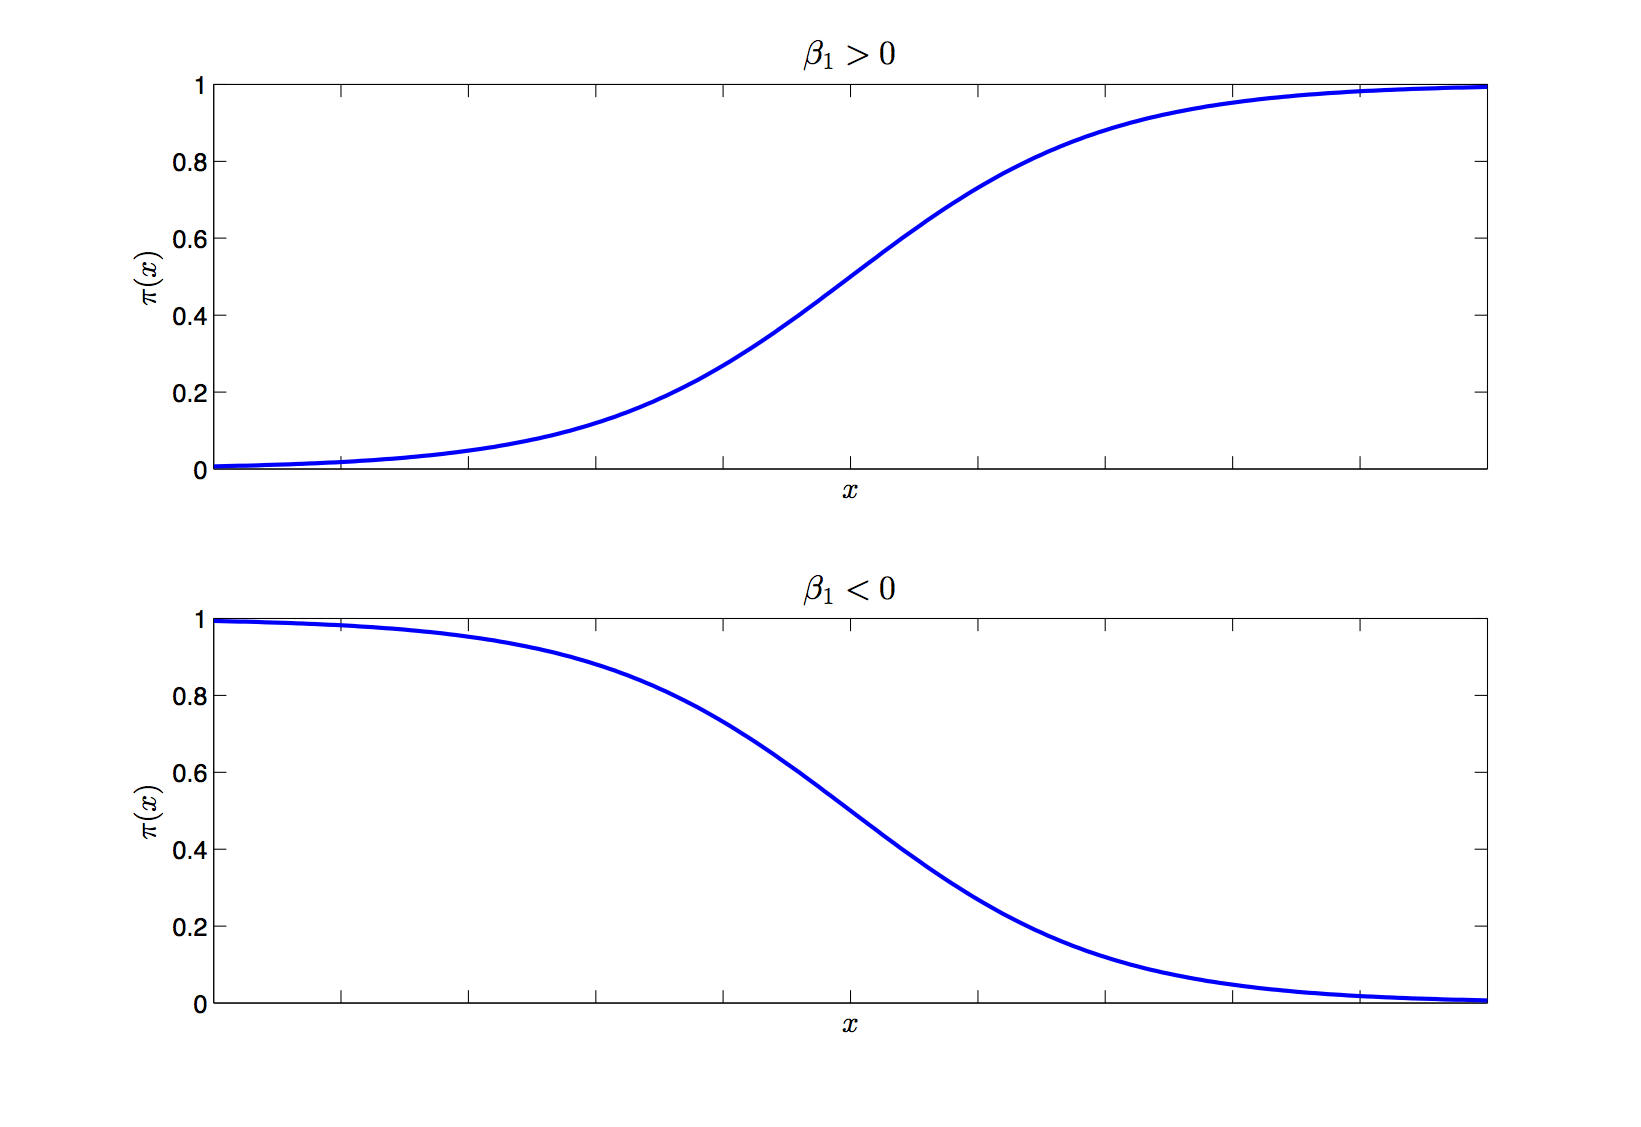
\includegraphics[width=0.45\textwidth]{logit.png}
    \end{center}
    }
    
    \only<2>{
    
    \bigskip
    
    \begin{itemize}
    \item $\hat{\pi}\left(x\right) = g^{-1}\left(\beta_0 + \beta_1x\right)$ принимает значения из $[0,1];$
    \item изменения на краях диапазона значений $x$ приводят к меньшим изменениям $\pi(x)$:
          $x$~--- годовой доход, $y$~--- покупка автомобиля,
          $$\hspace*{-0.5cm} \pi\left(10\,000\,000 + 200\,000\right) - \pi\left(10\,000\,000\right) < \pi\left(500\,000 + 200\,000\right) - \pi\left(500\,000\right).$$
    \end{itemize}    
    }
\end{frame}

\subsection{Интерпретация}
\begin{frame}{Отношение шансов}
    Пусть $y\sim Ber(p)$, тогда шансы (odds) события $y=1$: $$ODDS = \frac{p}{1-p}.$$

    \bigskip

    Если $y_1\sim Ber(p_1), \; y_2\sim Ber(p_2)$, то отношение шансов (odds ratio) события $y_1=1$ по сравнению с событием $y_2=1$: $$OR = \frac{p_1 / \left(1-p_1\right)}{p_2 / \left(1-p_2\right)}.$$

    \bigskip

    \begin{center}
    \begin{tabular}{|c|c|c|}
        \hline
        \diagbox{Серд. заболевания}{Возраст} &$\geq55$  &$<55$ \\\hline
        есть                                      &$21$ &$22$ \\\hline
        нет                                       &$6$  &$51$ \\\hline
    \end{tabular}
    \end{center}
    $$OR = \frac{21/6}{22/51}\approx 8.1.$$
\end{frame}

\begin{frame}{Роль коэффициентов логистической регрессии}
	

	
    $$\hat{g}\left(x\right) = \hat{\beta}_0 + \hat{\beta}_1 x \quad \Longleftrightarrow  \quad  \dfrac{p}{1-p} = e^{\hat{\beta}_0}  (e^{\hat{\beta}_1})^x  $$
	

    \bigskip

    Пусть $x = \left[\text{возраст}\geq55\right]$, \; $y=\left[\text{есть сердечные заболевания}\right].$
    По $\hat{\beta}_1$ легко оценить отношение шансов получения заболевания пожилыми людьми: $$\widehat{OR} = e^{\hat{\beta}_1}.$$

    \bigskip

    Пусть $x = \text{возраст}$, \; $y=\left[\text{есть сердечные заболевания}\right].$
    $e^{\hat{\beta}_1}$ имеет смысл мультипликативного прироста риска получения заболевания при увеличении возраста на 1 год.
\end{frame}

\subsection{Настройка параметров}
\begin{frame}{Настройка параметров}
    ММП:
%    
%    $\pi\left(x\right)$ оценивает $P\left(y=1\left|x\right.\right)$,
%
%    $1-\pi\left(x\right)$ оценивает $P\left(y=0\left|x\right.\right) \; \Rightarrow$
%
    \begin{align*}
    P\left(x_i,1\right) &= \pi\left(x_i\right), \\
    P\left(x_i,0\right) &= 1-\pi\left(x_i\right), \\
    l\left(\beta\right) &= \prod\limits_{i=1}^n \pi\left(x_i\right)^{y_i} \left(1-\pi\left(x_i\right)\right)^{1-y_i}, \\
    L\left(\beta\right) &= \ln l\left(\beta\right) = \sum\limits_{i=1}^n \left(y_i \ln \pi\left(x_i\right) + \left(1-y_i\right) \ln \left(1-\pi\left(x_i\right)\right)\right), \\
    \hat{\beta}         &= \argmax{\beta} L\left(\beta\right).
    \end{align*}
    
    \bigskip
    
    Информационная матрица Фишера:
    $$I\left(\hat{\beta}\right) = X^T V X, $$
    $$V=\diag\left(\hat{\pi}\left(x_i\right)\left(1-\hat{\pi}\left(x_i\right)\right)\right).$$
\end{frame}

% https://medium.datadriveninvestor.com/firths-logistic-regression-classification-with-datasets-that-are-small-imbalanced-or-separated-49d7782a13f1
\begin{frame}{Проблемы настройки параметров}
\only<1>{
	Если матрица $X$ вырождена, некоторые коэффициенты модели не будут определены. 
	
	\bigskip

	Если наблюдения $y=0$ и $y=1$ линейно разделимы в пространстве $X$, то:
	\begin{itemize}
	\item в теории коэффициенты бесконечно возрастают
	\item на практике коэффициенты и их дисперсии получаются большими, а~почти все вероятности в обучающей выборке близки к 0 или 1.
	\end{itemize}
	
	
	Можно использовать  регуляризацию Фирта. 
	Функция меток исходной модели для коэффициента $\beta_j$: $$\sum\limits_{i=1}^{n}\left(y_i - \pi\left(x_i\right)\right)x_{ij}.$$ 
	Регуляризованная версия: $$\sum\limits_{i=1}^{n}\left(y_i - \pi\left(x_i\right) + h_i\left(0.5-\pi\left(x_i\right)\right)\right)x_{ij},$$ 
	$h_i$~--- диагональный элемент hat matrix: $$H = V^{1/2}X\left(X^TVX\right)^{-1}X^TV^{1/2}.$$
}
\only<2>{
		\begin{center}
			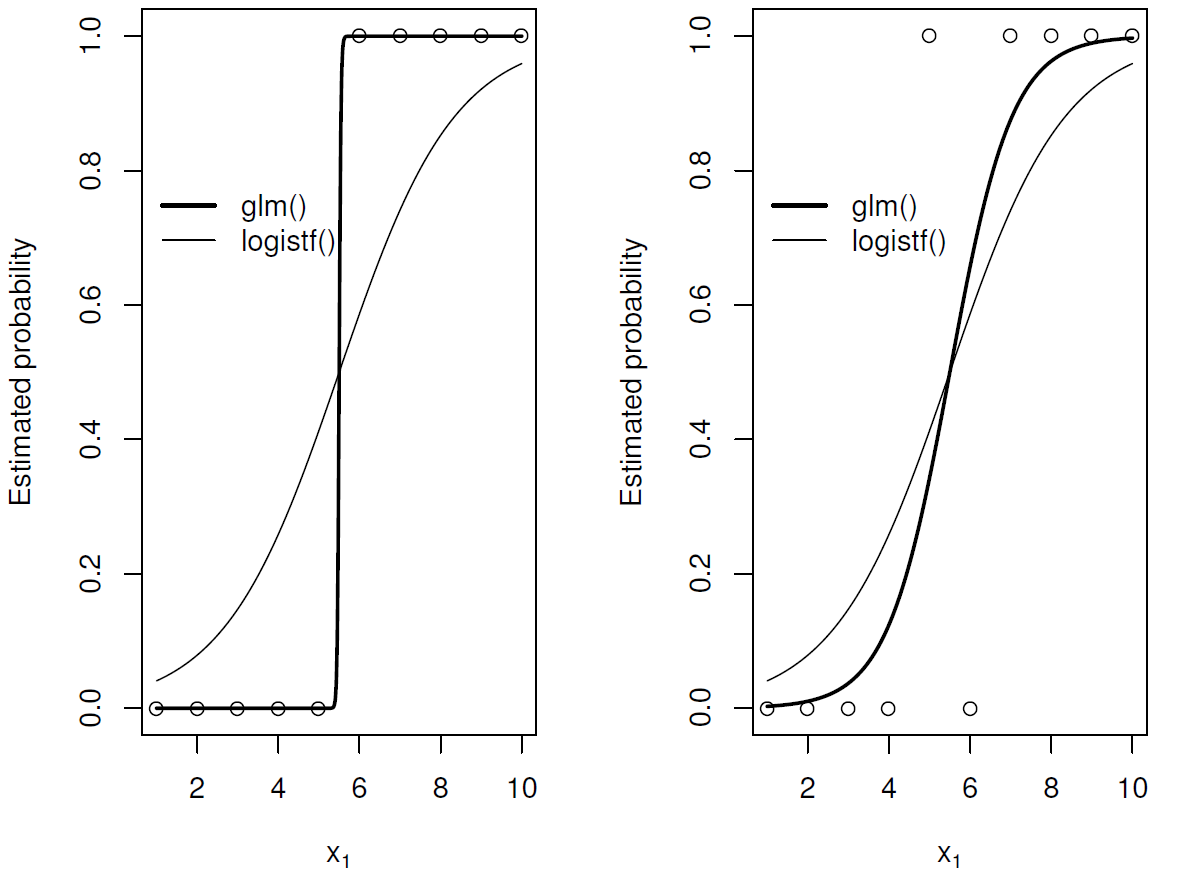
\includegraphics[width=0.65\textwidth]{separation.png}
		\end{center}	
	
}

\end{frame}

\begin{frame}{Доверительные интервалы}
    Для отдельного коэффициента $\beta_j$:
    $$\hat{\beta}_j \pm z_{1-\alpha/2} \sqrt{\left(I^{-1} \left(\hat{\beta}\right)\right)_{jj}}.$$

    \bigskip

    Для $g(x_0)$~--- логита нового объекта $x_0$:
    $$x_0^T \hat{\beta} \pm z_{1-\alpha/2} \sqrt{x_0^T I^{-1}\left(\hat{\beta}\right) x_0}.$$

    \bigskip

    Для вероятности $y=1$ при $x=x_0$:
    $$\left[\frac{e^{x_0 \hat{\beta} - z_{1-\alpha/2} \sqrt{x_0^T I^{-1}\left(\hat{\beta}\right) x_0}}}{1+e^{x_0 \hat{\beta} - z_{1-\alpha/2} \sqrt{x_0^T I^{-1}\left(\hat{\beta}\right) x_0}}}, \frac{e^{x_0 \hat{\beta} + z_{1-\alpha/2} \sqrt{x_0^T I^{-1}\left(\hat{\beta}\right) x_0}}}{1+e^{x_0 \hat{\beta} + z_{1-\alpha/2} \sqrt{x_0^T I^{-1}\left(\hat{\beta}\right) x_0}}}\right].$$
\end{frame}

\subsection{Линейность логита}
\begin{frame}{Линейность логита}
    Проверка линейности логита по признакам~--- аналог визуального анализа остатков в обычной линейной регрессии.

    \bigskip

    Методы анализа линейности логита:
    \begin{itemize}
    \item сглаженные диаграммы рассеяния;
%    \item фиктивные переменные по квартилям;
    \item дробные полиномы.
    \end{itemize}
\end{frame}

\begin{frame}{Сглаженные диаграммы рассеяния (smoothed scatterplots, LOESS)}
    Рассмотрим оценку логита, полученную ядерным сглаживанием по $x_j$:
     \begin{align*}
     \bar{y}_{sm}\left(x_{ji}\right) &= \frac{\sum\limits_{l=1}^n y_i K\left(\frac{x_{ji}-x_{li}}{h}\right)}{\sum\limits_{l=1}^n K\left(\frac{x_{ji}-x_{li}}{h}\right)}, \\
     \bar{l}_{sm}\left(x_{ji}\right) &= \ln \frac{\bar{y}_{sm}\left(x_{ji}\right)}{1-\bar{y}_{sm}\left(x_{ji}\right)}.
     \end{align*}

     \bigskip

     График функции $\bar{l}_{sm}\left(x_{j}\right) $ должен быть похож на прямую.
\end{frame}

%\begin{frame}{Фиктивные переменные по квартилям (design variables)}
%    \begin{enumerate}
%    \item Вычисляются выборочные квартили признака $x_j$: $\left[x_{j, 0.25}, x_{j, 0.5}, x_{j, 0.75}\right]$.
%    \item Создаются три фиктивные переменные:
%            \begin{align*}
%            D_{1i} &= \left[x_{j, 0.25} \leq x_{ji} < x_{j, 0.5}\right], \\
%            D_{2i} &= \left[x_{j, 0.5} \leq x_{ji} < x_{j, 0.75}\right], \\
%            D_{3i} &= \left[x_{j, 0.75} \leq x_{ji}\right].
%            \end{align*}
%    \item Настраивается логистическая регрессия, содержащая $D_1, D_2$ и $D_3$ вместо $x_j$. Пусть $\hat{\theta}_1,$ $\hat{\theta}_2$, $\hat{\theta}_3$~--- оценки коэффициентов при них.
%    \item Строится график, на котором середины интервалов, ограниченных квартилями, отложены против $\left[0, \hat{\theta}_1,\hat{\theta}_2, \hat{\theta}_3\right].$
%    \end{enumerate}
%\end{frame}

\begin{frame}{Дробные полиномы (fractional polynomials)}
    Если логит нелинеен по признаку, можно попробовать добавлять в модель его осмысленные степени и проверять их значимость.

    В автоматическом режиме это можно делать с помощью дробных полиномов.
    \begin{enumerate}
    \item Настраиваются модели с заменой $x_j$ на допустимые степени признака $x_j,$ например, из множества $S = \{{-2,-1,-0.5, 0, 0.5, 1, 2, 3}\}.$ Выбирается степень, максимизирующая правдоподобие.
    \item Настраиваются модели с заменой $x_j$ на двухкомпонентный полином $x_j$ вида $\beta_{j_1}x_j^{p_1} + \beta_{j_2}x_j^{p_2},$ \; $p_1,p_2\in S$ (если $p_1=p_2$, то берётся $\beta_{j_1}x_j^{p_1} + \beta_{j_2}x_j^{p_1}\ln x_j$). Выбираются степени, максимизирующие правдоподобие.
    \item Если модель с полиномом второй степени значимо не лучше, чем линейная, используется линейная модель.
    \item Если модель с полиномом второй степени значимо не лучше, чем с~полиномом первой степени, используется модель с полиномом первой степени, иначе~--- с полиномом второй.
    \end{enumerate}
\end{frame}

\subsection{Отбор признаков}
\begin{frame}{Содержательный отбор признаков}
    \only<1>{
    \begin{enumerate}
    \item Если признаков достаточно много (например, больше~10), желательно сделать их предварительный отбор, основанный на~значимости в~однофакторной логистической регрессии. Для дальнейшего рассмотрения остаются признаки, достигаемый уровень значимости которых не превышает~$0.25$.
    \item Строится многомерная модель, включающая все отобранные на~шаге~1 признаки. Проверяется значимость каждого признака, удаляется небольшая группа незначимых признаков. Новая модель сравнивается со старой с помощью критерия отношения правдоподобия.
    \item К признакам модели, полученной в результате циклического применения шагов~2 и~3, по одному добавляются удалённые признаки. Если какой-то из них становится значимым, он вносится обратно в~модель.    
    \end{enumerate}
    }

    \only<2>{
    \begin{enumerate}
    \setcounter{enumi}{3}
    \item Для непрерывных признаков полученной модели проверяется линейность логита. В случае обнаружения нелинейности признаки заменяются на соответствующие полиномы.
    \item Исследуется возможность добавления в полученную модель взаимодействий факторов. Добавляются значимые интерпретируемые взаимодействия.
    \item Проверяется адекватность финальной модели: близость $y$ и $\hat{y}$; малость вклада наблюдений $\left(x_i, y_i\right)$ на каждом объекте $i$ в $\hat{y}$.
    \end{enumerate}
    }
\end{frame}

\subsection{Классификация}
\begin{frame}{Порог классификации}
    \only<1>{
    Как по $\pi\left(x\right)$ оценить $y$?

    $$y = \left[\pi\left(x\right)\geq p_0\right].$$

    \bigskip

    Чаще всего берут $p_0=0.5$, но можно выбирать по другим критериям, например, для достижения заданных показателей чувствительности или~специфичности.
    }

    \only<2>{
    \textbf{Пример}: тест на вирус, $p_0=0.5$:

    \bigskip

    \begin{center}
    \begin{tabular}{|c|c|c|}
        \hline
        \diagbox{$\hat{y}$}{$y$} &$1$   &$0$ \\\hline
        $1$                           &$16$  &$11$ \\\hline
        $0$                           &$131$ &$417$ \\\hline
    \end{tabular}
    \end{center}

    \bigskip

    Чувствительность: $\frac{tp}{tp+fn} = \frac{16}{16+131} \approx 10.9\%.$

    Специфичность: $\frac{tn}{fp+tn} = \frac{417}{11+417} \approx 97.4\%.$

    \begin{center}
        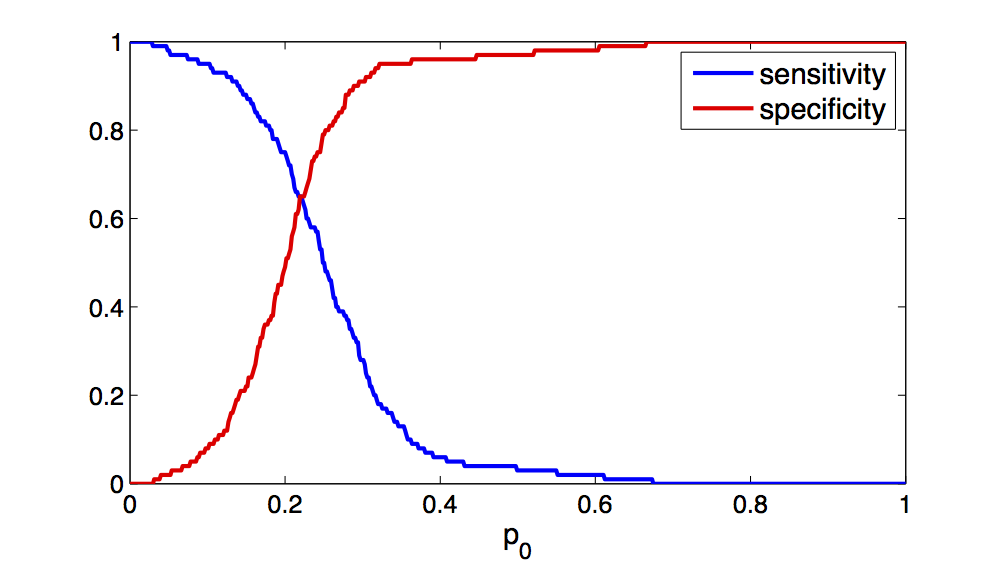
\includegraphics[width=0.5\textwidth]{drugs.png}
    \end{center}
    }
    \only<3>{
    
    \begin{center}
        Полнота = Чувствительность: $\frac{tp}{tp+fn}.$

        Точность: $\frac{tp}{fp+fp}.$

        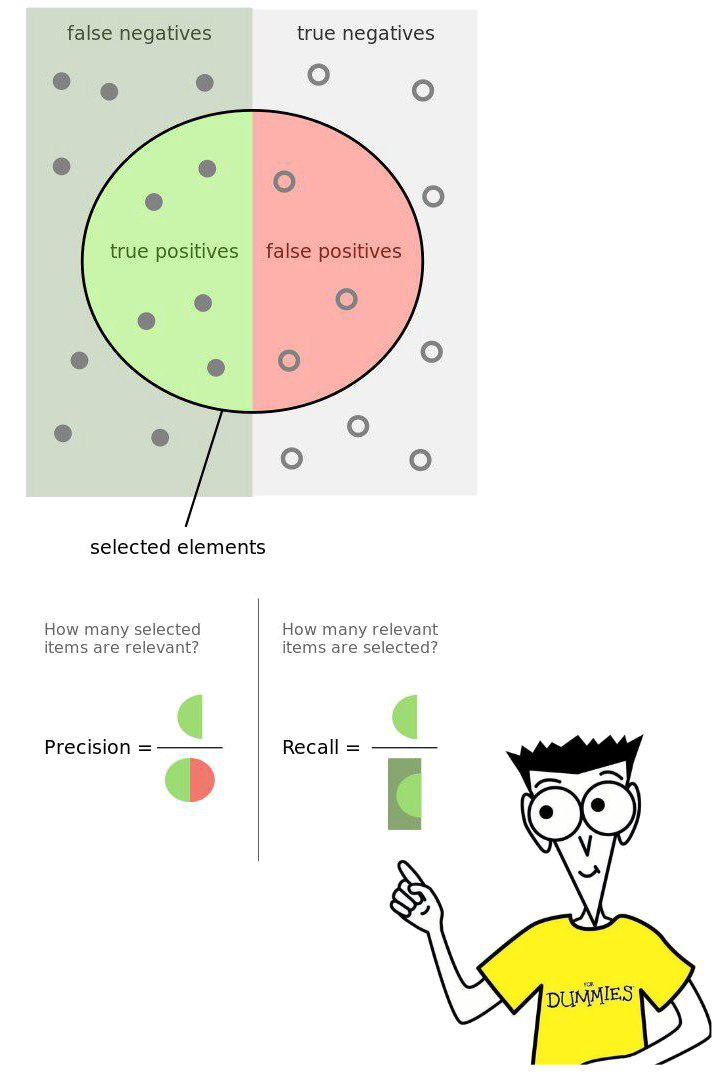
\includegraphics[width=0.25\textwidth]{dummies.png}
    \end{center}
    }
\end{frame}
%
%\subsection{Выбросы}
\begin{frame}{Выбросы}
    Остатки Пирсона:
    $$r_i = \frac{y_i-\hat{\pi}\left(x_i\right)}{\sqrt{\hat{\pi}\left(x_i\right)\left(1-\hat{\pi}\left(x_i\right)\right)}}.$$

    Аналог расстояния Кука:
    $$\Delta\hat{\beta}_i = \frac{r^2_{i} h_i}{\left(1-h_i\right)^2}.$$
\end{frame}

%\subsection{Пример}
%\begin{frame}{Пример}
%%	Риск остеопоротических переломов у женщин:
%%	
%%	\url{https://yadi.sk/d/fkjAG2StfJm4J}
%
%	Задача интерпретации кардиотокографии:
%	
%	\url{https://yadi.sk/d/n4EKlhNwfnM3p}
%\end{frame}

\subsection{Итог}
\begin{frame}
    \frametitle{Требования к решению задачи методом логистической регрессии}
    \begin{itemize}
    \item визуализация данных, оценка наличия выбросов, анализ таблиц сопряжённости по категориальным признакам;
    \item содержательный отбор признаков: выбор наилучшей линейной модели, оценка линейности непрерывных признаков по логиту, анализ необходимости добавления взаимодействий, проверка адекватности финальной модели (анализ влиятельных наблюдений, классификация);
    \item выводы.
    \end{itemize}
\end{frame}

\section{Натуральный отклик}
\subsection{Постановка}
\begin{frame}{Натуральный отклик: постановка задачи}
	$1,\dots,n$~--- объекты;
	
	$x_1,\dots,x_k$~--- предикторы;
	
	$y$~--- счётный отклик, $y_i \in \mathbb{N}$.
	
	$$\mathbb{E}\left(y\left|x\right.\right)=?$$
	
	\bigskip
	
	Базовый метод~--- пуассоновская регрессия:
	\begin{align*}
	f\left(y\left|x\right.\right)          &= \frac{e^{-\mu}\mu^y}{y!}, \\
	\mu                                    &= \mathbb{E}\left(y\left|x\right.\right) = e^{x^T\beta}, \\
	\omega                                 &\equiv \mathbb{D}\left(y\left|x\right.\right) = e^{x^T\beta}.
	\end{align*}
\end{frame}

\begin{frame}{Примеры}
	Стандартная пуассоновская модель: 
	
	$x_{ij}$~--- макроэкономические показатели, $y_i$~--- число банкротств банков, $$\ln \mu = X\beta.$$
	
	\bigskip
	
	Может использоваться также для нормированных данных: 
	
	$N_i$~--- общее число банков, $\frac{1000y_i}{N_i}$~--- число банкротств на 1000 банков,
	$$\ln \frac{1000\mu}{N} = X\beta, \;\; \ln \mu = \ln \frac{N}{1000} + X\beta.$$
\end{frame}



\subsection{Настройка параметров}
\begin{frame}{Настройка параметров}
	ММП:
	\begin{align*}
	l\left(\beta\right) &= \prod_{i=1}^n \frac{e^{-e^{x^T\beta}} \left(e^{x^T\beta}\right)^{y_i}}{y_i!},\\
	L\left(\beta\right) &= \ln l\left(\beta\right) = \sum\limits_{i=1}^n \left( y_i x_i^T\beta - e^{x_i^T\beta} - ln \left(y_i!\right)\right), \\
	\hat{\beta}         &= \argmax{\beta} L\left(\beta\right) \Leftrightarrow \\
	& \sum_{i=1}^n \left(y_i - e^{x_i^T\beta}\right)x_i = 0.
	\end{align*}
\end{frame}

%\begin{frame}{Отличия от линейной модели}
%	$$\hat{\beta} = $$
%
%	\bigskip
%	
%	При настройке обычной линейной регрессии с логарифмом отклика $$\hat{\beta} = \argmin_{\beta}{\sum_{i=1}^n \left(\ln y_i - x_i^T\beta\right)}$$
%\end{frame}

\subsection{Доверительные интервалы}
\begin{frame}{Доверительные интервалы}
	Для отдельного коэффициента $\beta_j$:
	$$\hat{\beta}_j \pm z_{1-\alpha/2} \sqrt{\left(I^{-1} \left(\hat{\beta}\right)\right)_{jj}}.$$
	
	Для $\ln\mathbb{E}\left(y\left|\right.x=x_0\right)=x_0^T\beta$:
	$$x_0^T \hat{\beta} \pm z_{1-\alpha/2} \sqrt{x_0^T I^{-1}\left(\hat{\beta}\right) x_0}.$$
	
	Для $\mathbb{E}\left(y\left|\right.x=x_0\right)=e^{x_0^T\beta}$:
	$$\left[e^{x_0^T \hat{\beta} - z_{1-\alpha/2} \sqrt{x_0^T I^{-1}\left(\hat{\beta}\right) x_0}}, e^{x_0^T \hat{\beta} + z_{1-\alpha/2} \sqrt{x_0^T I^{-1}\left(\hat{\beta}\right) x_0}}\right].$$
	
	Приближённый предсказательный интервал для $y\left(x_0\right)$~--- отклика на новом объекте $x_0$:
	$$e^{x_0^T\hat{\beta}} \pm 2\sqrt{e^{x_0^T\hat{\beta}}}.$$
\end{frame}

\subsection{Равенство матожидания и дисперсии}
\begin{frame}{Overdispersion/underdispersion}
	\only<1>{
		Пуассоновская модель предполагает, что $\omega=\mu$ (equidispersion).
		
		\bigskip
		
		\begin{itemize}
			\item МП-оценки $\beta$ остаются состоятельными, даже если распределение $y|x$ не является пуассоновским~--- достаточно того, что модель $\mathbb{E}\left(y\left|x\right.\right)$ определена корректно.
			\item Оценки дисперсии $\hat{\beta}$ и соответствующие критерии требуют верного определения и $\mathbb{D}\left(y\left|x\right.\right)$, поэтому они дают некорректные результаты, если матожидание и дисперсия не равны.
			\item Предположение о равенстве матожидания и дисперсии можно проверить; если оно не выполняется, можно изменить модель. Это~позволит построить корректные критерии и более эффективные оценки $\beta$.
		\end{itemize}
	}
	\only<2>{
		Overdispersion~--- отрицательная биномиальная модель:
		\begin{align*}
		\omega\left(\alpha\right) & =\mu+\alpha\mu^2, \\
		f\left(y\left|\mu,\alpha\right.\right) &= \frac{\Gamma\left(y+\alpha^{-1}\right)}{\Gamma\left(y+1\right) \Gamma\left(\alpha^{-1}\right)} \left( \frac{\alpha^{-1}}{\alpha^{-1}+\mu} \right)^{\alpha^{-1}} \left(\frac{\mu}{\alpha^{-1}+\mu}\right)^y.
		\end{align*}
		
		\bigskip
		
		Underdispersion~--- пороговая модель (hurdle model):
		$$P\left(y=j\right) = \begin{cases}
		f_1\left(0\right), & j=0, \\
		\frac{1-f_1\left(0\right)}{1-f_2\left(0\right)}f_2\left(j\right), & j>0.
		\end{cases}
		$$
		
		\bigskip
		
		Можно построить МП-оценки для $\alpha$ и $\beta$, а затем проверить гипотезу $\alpha=0$ с помощью критерия отношения правдоподобия.
	}
\end{frame}

\begin{frame}{Устойчивая оценка дисперсии}
	Дисперсия оценки максимального квазиправдоподобия:
	$$\mathbb{D}_{QML}\left(\hat{\beta}\right) = \left( \sum\limits_{i=1}^n \mu_i x_i x_i^T\right)^{-1} \left( \sum\limits_{i=1}^n \omega_i x_i x_i^T\right) \left( \sum\limits_{i=1}^n \mu_i x_i x_i^T \right)^{-1}. $$
	
	\bigskip
	
	Устойчивая состоятельная оценка дисперсии, подходящая для любого вида $\omega$:
	$$\mathbb{D}_{R}\left(\hat{\beta}\right) = \left( \sum\limits_{i=1}^n \mu_i x_i x_i^T\right)^{-1} \left( \sum\limits_{i=1}^n \left(y_i-\mu_i\right)^2 x_i x_i^T\right) \left( \sum\limits_{i=1}^n \mu_i x_i x_i^T \right)^{-1}. $$
\end{frame}

\subsection{Меры качества модели}
\begin{frame}{Меры качества модели}
	Относительные:
	\begin{itemize}
		\item аномальность:
		\begin{align*}
		D_P    &= \sum\limits_{i=1}^n \left( y_i \ln \frac{y_i}{\hat{\mu}_i} - \left(y_i-\hat{\mu}_i \right) \right), \\%
		D_{NB} &= \sum\limits_{i=1}^n \left( y_i \ln \frac{y_i}{\hat{\mu}_i} - \left(y_i+\alpha^{-1}\right)\ln \frac{y_1 + \alpha^{-1}}{\hat{\mu}_i + \alpha^{-1}} \right);
		\end{align*}
		\item AIC: $$AIC = -2L +2\left(k+1\right).$$
	\end{itemize}
	
	\bigskip
	
	Абсолютная:
	\begin{itemize}
		\item псевдо-$R^2$:
		$$R^2_{DEV} = 1-\frac{D}{D_0},$$
		$D_0$~--- аномальность модели с одной константой.
	\end{itemize}
\end{frame}

%\subsection{Пример}
%\begin{frame}{Пример}
%	Число визитов к доктору:
%	
%	\url{https://yadi.sk/d/iaB-RbvRfNcC3}
%\end{frame}

\subsection{Итог}
\begin{frame}
	\frametitle{Требования к решению задачи методом пуассоновской регрессии}
	\begin{itemize}
		\item визуализация данных, оценка наличия выбросов;
		\item отбор признаков: выбор наилучшей линейной модели, проверка равенства среднего и дисперсии, анализ необходимости добавления взаимодействий, проверка адекватности финальной модели (сравнение с устойчивой моделью, анализ влиятельных наблюдений);
		\item выводы.
	\end{itemize}
\end{frame}

\section{}
\begin{frame}
\frametitle{Литература}    
    \begin{itemize}
    \item обработка пропусков~--- Gu;
    \item обобщённые линейные модели~--- Olsson;
    \item логистическая регрессия~--- Bilder, глава 2, Hosmer;
    \item регрессия на счётных данных~--- Bilder, глава 4, Cameron.
    \end{itemize}
    
    \bigskip
    
    Bilder, C.R., Loughin, T.M. Analysis of Categorical Data with R, 2013.
    		
    		\vspace{5pt}    
    		        		
	Cameron C.A., Trivedi P.K. \textit{Regression Analysis of Count Data}, 2013.   
    		
    		\vspace{5pt}    
    		        		
    Gu X.M. \textit{A Different Approach to the Problem of Missing Data}. In Joint Statistical Meetings, 2015, Seattle, WA. 
        		
        	\vspace{5pt}    			
    		
    Hosmer D.W., Lemeshow S., Sturdivant R.X. \textit{Applied Logistic Regression}, 2013. 
    		
    		\vspace{5pt}    		
    		
	Olsson U. {\em Generalized Linear Models: An Applied Approach}, 2004.
\end{frame}

\end{document}
